\app{} brings the drawing, the equipment data, the protection zones and the
calculation together in one window. The zones and results are worked out from the
drawing itself, so they always match it.

\subsection{Capabilities}

\begin{description}[style=nextline, leftmargin=1.2em]
  \item[Equipment library]
    Define each type of equipment once with \ui{Create Component}, choosing from 13
    symbol types and entering its electrical data. It then appears in the Equipment
    Library, and you drag copies onto the drawing.
  \item[Drawing workspace]
    A grid-aligned canvas the size of a $48 \times 36$ inch drawing sheet. Place, wire,
    move, rotate and resize equipment; every edit can be undone.
  \item[PDF background]
    Show the first page of the original one-line PDF under the drawing, at true scale,
    and trace the station over it.
  \item[Validation]
    \ui{Validate} finds unconnected terminals, dangling wires and wiring shorts.
  \item[Protection zones]
    The tool proposes bus, transformer and line zones from the wiring and the CTs. You
    review each zone in the \ui{Configure Zones} dialog, assign the equipment that
    operates, and verify it.
  \item[Momentary load calculation]
    For each zone and stage, the tool adds up the currents that flow together on each
    DC supply. Each supply's largest total, across all verified zones, is its peak.
  \item[Reports and files]
    Save studies as layout files. Export a calculation report with the annotated
    one-line, and a netlist report listing every component and connection.
\end{description}

\subsection{Typical Workflow}

Figure~\ref{fig:workflow} shows the steps of a study. Steps~5 to~8 repeat whenever the
drawing or the zones change. Any edit clears the previous results, so an exported
report always matches the current drawing.

\begin{figure}[H]
  \centering
  \begin{tikzpicture}[
      node distance=6mm and 7mm,
      wstep/.style={rectangle, rounded corners=3pt, draw=gftgreen, line width=0.8pt,
                   fill=gftlight, align=center, font=\small, minimum height=12mm,
                   text width=30mm},
      arr/.style={-{Stealth[length=2.5mm]}, line width=0.8pt, color=gftgreen!80!black}]
    \node[wstep] (s1) {\textbf{1. New layout}\\Name the project};
    \node[wstep, right=of s1] (s2) {\textbf{2. Import PDF}\\Original one-line as background};
    \node[wstep, right=of s2] (s3) {\textbf{3. Build the one-line}\\Create, place and wire equipment};
    \node[wstep, below=of s3] (s4) {\textbf{4. Enter data}\\Currents, status, breaker settings};
    \node[wstep, left=of s4] (s5) {\textbf{5. Validate}\\Fix open ends and shorts};
    \node[wstep, left=of s5] (s6) {\textbf{6. Run Evaluation}\\Zones proposed};
    \node[wstep, below=of s6] (s7) {\textbf{7. Configure}\\\textbf{Zones}\\Assign loads, verify};
    \node[wstep, right=of s7] (s8) {\textbf{8. Review results}\\Zone outlines and totals};
    \node[wstep, right=of s8] (s9) {\textbf{9. Export}\\Calculation PDF and layout};
    \draw[arr] (s1) -- (s2);
    \draw[arr] (s2) -- (s3);
    \draw[arr] (s3) -- (s4);
    \draw[arr] (s4) -- (s5);
    \draw[arr] (s5) -- (s6);
    \draw[arr] (s6) -- (s7);
    \draw[arr] (s7) -- (s8);
    \draw[arr] (s8) -- (s9);
    \draw[arr, dashed] (s8.south) -- ++(0,-5mm) -| node[pos=0.25, below, font=\footnotesize]{edit and re-run} (s7.south);
  \end{tikzpicture}
  \caption{Typical workflow of a momentary DC load study}
  \label{fig:workflow}
\end{figure}

\subsection{The Main Window}

Figure~\ref{fig:mainwindow} shows the main window with a completed study open, and
Table~\ref{tab:mainwindow} describes each numbered area.

\begin{figure}[H]
  \centering
  \begin{tikzpicture}
    \node[anchor=south west, inner sep=0] (img) {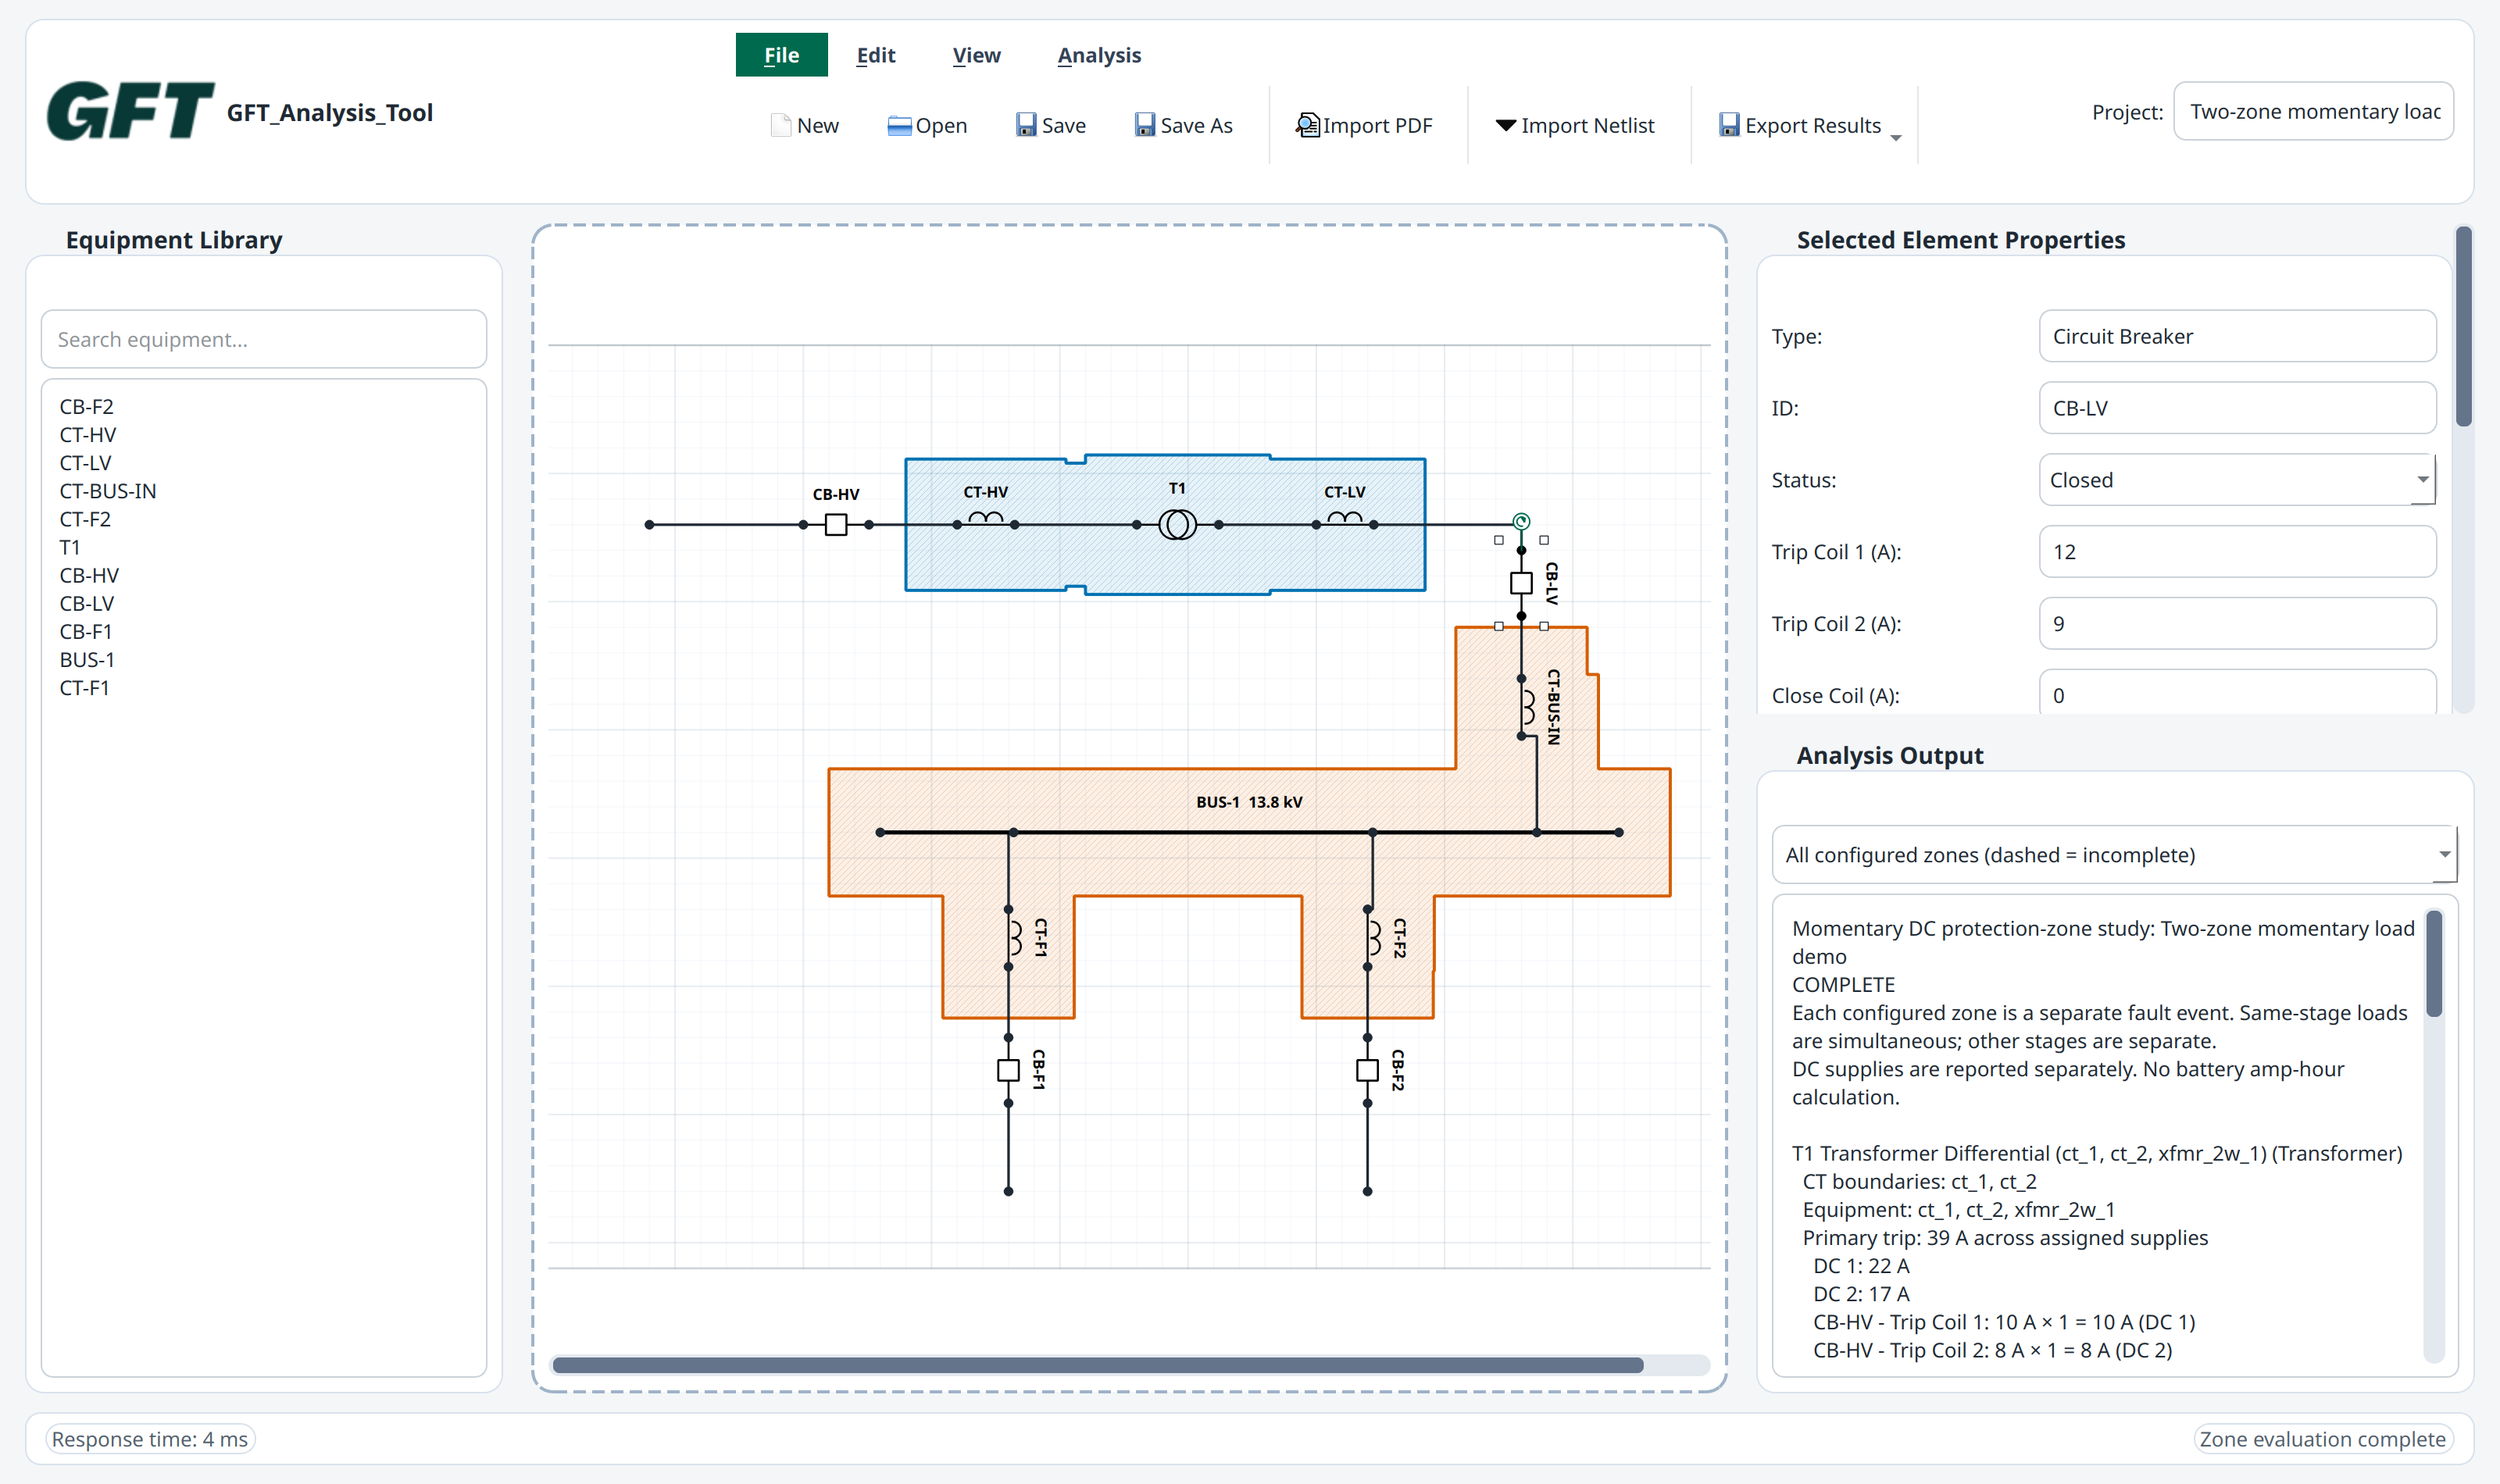
\includegraphics[width=\textwidth]{images/main_window.png}};
    \begin{scope}[x={(img.south east)}, y={(img.north west)},
        callout/.style={circle, fill=gftgreen, text=white, font=\small\bfseries,
                        inner sep=1.5pt, minimum size=5.5mm, draw=white, line width=0.8pt}]
      \node[callout] at (0.195, 0.925) {1};
      \node[callout] at (0.475, 0.963) {2};
      \node[callout] at (0.815, 0.925) {3};
      \node[callout] at (0.130, 0.838) {4};
      \node[callout] at (0.250, 0.790) {5};
      \node[callout] at (0.870, 0.838) {6};
      \node[callout] at (0.810, 0.491) {7};
      \node[callout] at (0.115, 0.030) {8};
    \end{scope}
  \end{tikzpicture}
  \caption{Main window with the two-zone demonstration study evaluated}
  \label{fig:mainwindow}
\end{figure}

\begin{table}[H]
  \centering
  \caption{Areas of the main window}
  \label{tab:mainwindow}
  \begin{tabularx}{\textwidth}{c l L}
    \toprule
    & \textbf{Area} & \textbf{Purpose} \\
    \midrule
    1 & Header & The GFT logo and the tool's name. \\
    2 & Ribbon & Commands, on the File, Edit, View and Analysis tabs (Section~\ref{sec:ribbon}). \\
    3 & Project field & The project name, which appears in the window title and the reports. \\
    4 & Equipment Library & The equipment available to place, with a search box. Drag an entry onto the drawing to place it. \\
    5 & Drawing workspace & The one-line diagram, the grid and the optional PDF background. Zone outlines appear here after an evaluation. \\
    6 & Selected Element Properties & The selected component's type, ID, status and electrical data. Breakers also show their breaker settings. \\
    7 & Analysis Output & A zone selector and the results of the last evaluation. \\
    8 & Status bar & How long the last evaluation took (left), and the last action or status message (right). \\
    \bottomrule
  \end{tabularx}
\end{table}

The window title shows the project name. An asterisk (*) after it means there are
unsaved changes.

\subsection{The Ribbon}\label{sec:ribbon}

The commands are on four tabs (Figure~\ref{fig:ribbon}). If the window is too narrow
to show a whole tab, its commands scroll sideways.

\begin{figure}[H]
  \centering
  \begin{subfigure}{\textwidth}\centering
    
\includegraphics[width=0.82\textwidth]{images/ribbon_file.png}\caption{File}\end{subfigure}\\[3pt]
  \begin{subfigure}{\textwidth}\centering
    
\includegraphics[width=0.82\textwidth]{images/ribbon_edit.png}\caption{Edit}\end{subfigure}\\[3pt]
  \begin{subfigure}{\textwidth}\centering
    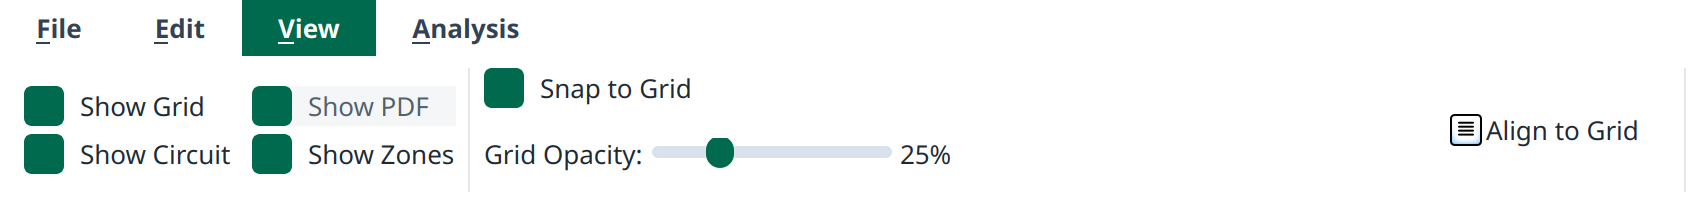
\includegraphics[width=0.82\textwidth]{images/ribbon_view.png}\caption{View}\end{subfigure}\\[3pt]
  \begin{subfigure}{\textwidth}\centering
    
\includegraphics[width=0.82\textwidth]{images/ribbon_analysis.png}\caption{Analysis}\end{subfigure}
  \caption{The four ribbon tabs}
  \label{fig:ribbon}
\end{figure}

\begin{table}[H]
  \centering
  \caption{Ribbon commands}
  \label{tab:ribbon}
  \begin{tabularx}{\textwidth}{l L}
    \toprule
    \textbf{Tab} & \textbf{Commands} \\
    \midrule
    File & New, Open, Save, Save As, Import PDF, Import Netlist, Export Results
           (calculation PDF or netlist PDF) \\
    Edit & Undo, Redo, Copy, Paste, Delete, Rotate 90°, Create Component \\
    View & Show Grid, Show PDF, Show Circuit, Show Zones, Snap to Grid, grid opacity,
           Align to Grid \\
    Analysis & Validate, Configure Zones, Run Evaluation, Expand Analysis \\
    \bottomrule
  \end{tabularx}
\end{table}

\subsection{Software Architecture}

\app{} is written in Python~3.12. It uses PySide6~\cite{pyside6}, the Python version
of the Qt toolkit, for its interface, and PyMuPDF~\cite{pymupdf} to read PDF
backgrounds. The code has two layers (Figure~\ref{fig:architecture}):
\begin{itemize}
  \item the \emph{GUI layer}: the windows, the drawing, the dialogs and the reports;
  \item the \emph{logic layer}: zone detection and the calculation, with no interface
        code.
\end{itemize}
Keeping the layers separate means the calculation can be tested on its own, without
opening a window.


\begin{figure}[H]
  \centering
  \begin{tikzpicture}[
      mod/.style={rectangle, draw=gftgreen, fill=white, rounded corners=2pt, font=\footnotesize\ttfamily,
                  minimum width=36mm, minimum height=6mm, align=center},
      layer/.style={rectangle, draw=gftgreen!60, fill=gftlight, rounded corners=4pt, inner sep=3mm},
      lbl/.style={font=\small\bfseries, color=gftgreen!80!black},
      file/.style={rectangle, draw=notegrey, fill=gray!8, font=\footnotesize, minimum width=30mm,
                   minimum height=6mm, align=center},
      arr/.style={-{Stealth[length=2mm]}, line width=0.7pt, color=notegrey}]
    % GUI layer
    \node[mod] (main) {substation\_gui};
    \node[mod, right=4mm of main] (ws) {workspace};
    \node[mod, right=4mm of ws] (zd) {zone\_dialog};
    \node[mod, below=2mm of main] (ev) {evaluation\_view};
    \node[mod, below=2mm of ws] (sym) {symbols, routing};
    \node[mod, below=2mm of zd] (ol) {operating\_loads};
    \node[mod, below=2mm of ev] (pf) {project\_files, layout\_io};
    \node[mod, below=2mm of sym] (cmd) {commands};
    \node[mod, below=2mm of ol] (cc) {custom\_widget\_tool};
    \node[mod, below=2mm of pf] (pdf) {pdf\_export};
    \node[mod, below=2mm of cmd] (chk) {circuit\_check};
    \node[mod, below=2mm of cc] (rib) {ribbon, theme, messages};
    \begin{scope}[on background layer]
      \node[layer, fit=(main)(rib)(pdf), label={[lbl]above:GUI layer (gui/): windows, canvas, dialogs, reports}] (gui) {};
    \end{scope}
    % Logic layer
    \node[mod, below=24mm of pdf] (pz) {protection\_zones};
    \node[mod, right=4mm of pz] (ps) {protection\_study};
    \node[mod, right=4mm of ps] (bs) {breaker\_settings};
    \node[mod, below=2mm of pz] (mc) {momentary\_calc2};
    \node[mod, below=2mm of ps] (nm) {netlist\_manager};
    \begin{scope}[on background layer]
      \node[layer, fit=(pz)(bs)(nm), label={[lbl]above:Logic layer (logic/): no user-interface code}] (logic) {};
    \end{scope}
    \draw[arr] (gui.south) -- ([yshift=6mm]logic.north) node[midway, right=1mm, font=\footnotesize, text=notegrey]{netlist and zone settings};
    % Files read and written by the GUI layer
    \node[file, right=9mm of zd] (lay) {Layout file (.json)};
    \node[file, below=2mm of lay] (bg) {One-line PDF};
    \node[file, below=2mm of bg] (rep) {Report PDFs};
    \node[file, below=2mm of rep] (net) {Netlist (.json)};
    \node[font=\footnotesize\bfseries, color=notegrey, above=1mm of lay] {Files};
    \draw[arr, {Stealth[length=2mm]}-{Stealth[length=2mm]}] (gui.east |- lay) -- (lay.west);
    \draw[arr] (bg.west) -- (gui.east |- bg);
    \draw[arr] (gui.east |- rep) -- (rep.west);
    \draw[arr] (net.west) -- (gui.east |- net);
  \end{tikzpicture}
  \caption{Software structure. The GUI layer turns the drawing into a netlist and passes it, with the zone settings, to the logic layer.}
  \label{fig:architecture}
\end{figure}

\begin{table}[H]
  \centering
  \caption{Main modules}
  \label{tab:modules}
  \begin{tabularx}{\textwidth}{l L}
    \toprule
    \textbf{Module} & \textbf{Responsibility} \\
    \midrule
    \texttt{protection\_zones} & Splits the drawing into regions bounded by CTs, following the wiring and taking open switches into account. \\
    \texttt{protection\_study} & Proposes zones, checks zone settings, calculates each zone's stages and supplies, and decides whether the study is complete. \\
    \texttt{breaker\_settings} & Works out each breaker coil's multiplier and DC supply from the breaker settings. \\
    \texttt{momentary\_calc2} & Adds up simultaneous currents. \\
    \texttt{netlist\_manager} & Builds and reads netlists (lists of components and connections). \\
    \texttt{substation\_gui} & The main window, the properties panel and the ribbon commands. \\
    \texttt{workspace}, \texttt{symbols}, \texttt{routing} & The drawing canvas, the equipment symbols and the right-angle wire routing. \\
    \texttt{commands} & Undo and redo for every edit. \\
    \texttt{zone\_dialog}, \texttt{operating\_loads} & The Configure Zones dialog and its operating-load rows. \\
    \texttt{project\_files}, \texttt{layout\_io} & Opening, saving and importing layouts and netlists. \\
    \texttt{pdf\_export} & The calculation and netlist PDF reports. \\
    \bottomrule
  \end{tabularx}
\end{table}

\subsection{Files Used and Produced}

Table~\ref{tab:files} lists the files the tool reads and writes.

\begin{table}[H]
  \centering
  \caption{Files used and produced by the tool}
  \label{tab:files}
  \begin{tabularx}{\textwidth}{l l L}
    \toprule
    \textbf{File} & \textbf{Created by} & \textbf{Contents} \\
    \midrule
    Layout (\texttt{.json}) & Save, Save As & The whole study: the equipment and its data, the drawing, the Equipment Library, the zones, and the path of the background PDF. \\
    One-line PDF & The utility & The original drawing, used as a background. The layout stores its path, not the PDF itself. \\
    Netlist (\texttt{.json}) & Another tool or script & Components and connections only. Importing one replaces the current drawing. \\
    Calculation PDF & Export Results & Supply peaks, a zone summary, review issues, the annotated one-line and the full results. \\
    Netlist PDF & Export Results & Every component, with its properties and connections. \\
    \bottomrule
  \end{tabularx}
\end{table}

Appendix~\ref{app:formats} describes the two JSON formats in detail.
